\chapter{Synthetische Rekonstruktion}
\label{sec:minimal} 

Anhand der erarbeiteten mathematischen Grundlagen ist ein Algorithmus für die Rekonstruktion einer Szene aus einer Stereobildaufnahme entstanden. Der Algorithmus wurde mit dem Ziel der Kamerakalibrierung und der Szenenrekonstruktion aus Bildquellen unterschiedlicher Auflösungen entwickelt, da Stereokalibrierungsverfahren einiger Computer Vision Applikationen keine unterschiedlichen Auflösungen von Kameras berücksichtigen. Der entwickelte Algorithmus ist in der Lage aus einem Stereobildpaar extrinsische Kameraparameter zu bestimmen und anhand dessen die 3D-Szene zu rekonstruieren, jedoch unter der Voraussetzung, dass die intrinsischen Kameraparameter beider Kameras bekannt sind.\\

Im Folgenden wird der Algorithmus anhand eines virtuellen Beispiels erklärt. Dabei werden die einzelnen Schritte des Aufbaus der virtuellen Szene, der Bestimmung der extrinsischen Kameraparameter und der Rekonstruktion der virtuellen 3D-Szene beschrieben. Abbildung \ref{fig:ArbeitsProzessVirtuell} fasst den Arbeitsprozess des Szenenrekonstruktionsalgorithmus für das virtuelle Beispiel zusammen. \\




\begin{figure}[!htb]%{\linewidth}
	\centering
	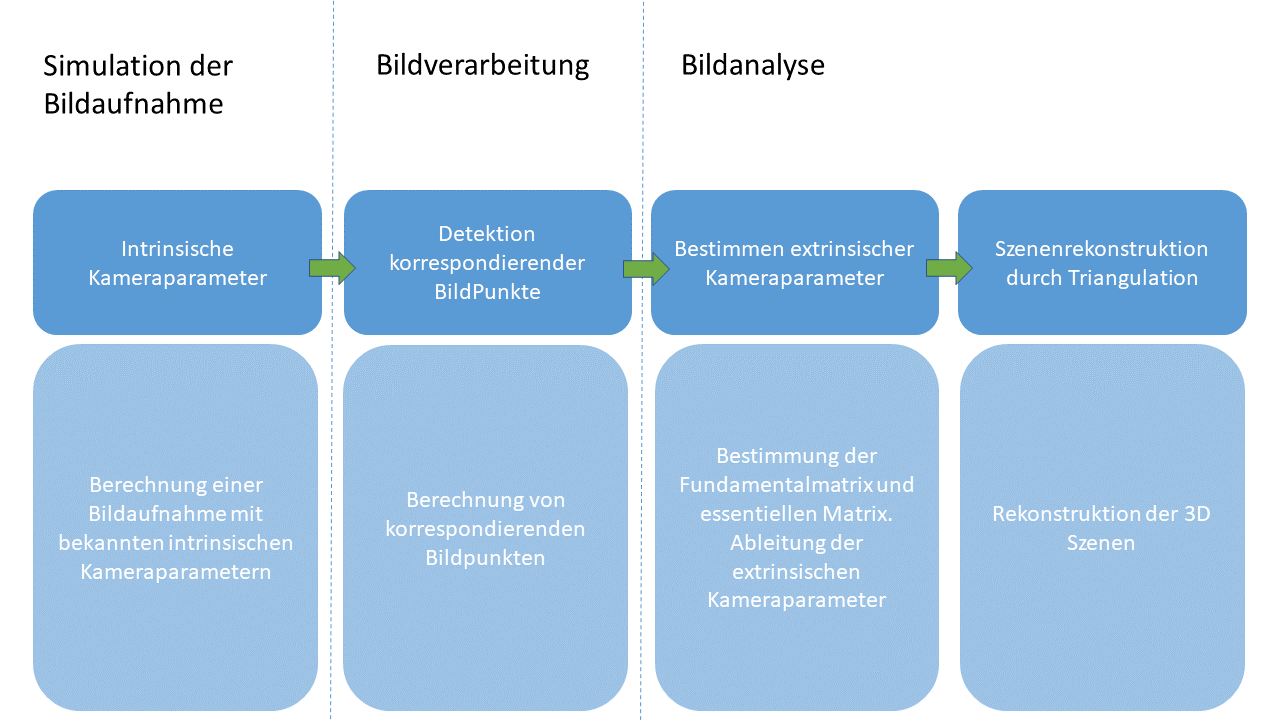
\includegraphics[width=1.\linewidth]{images/NEU_Virtuel_Arbeitsprozess.png}
	\caption[Ablaufdiagram]{Ablaufdiagramm für das synthetische Beispiel}
	\label{fig:ArbeitsProzessVirtuell}
\end{figure}

%\begin{figure}%{\linewidth}
%	\centering
%	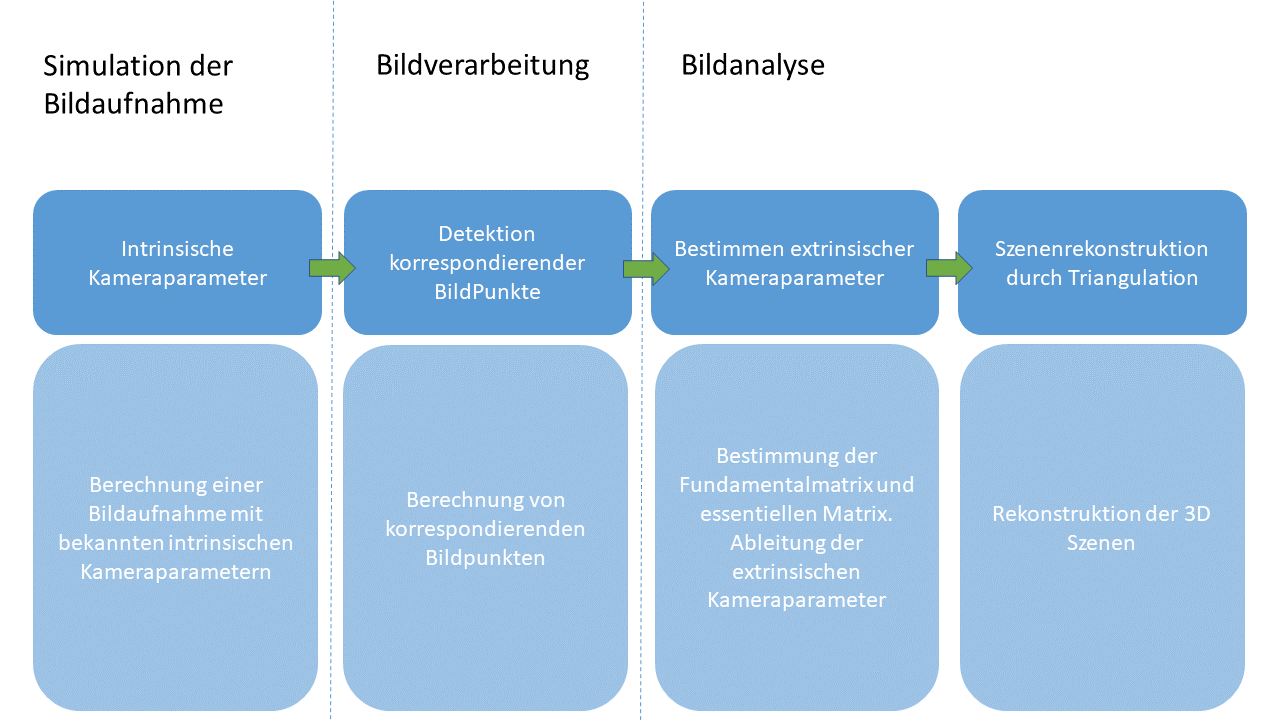
\includegraphics[width=0.8\linewidth]{images/NEU_Virtuel_Arbeitsprozess.png}
%	\caption[Ablaufdiagram]{Ablaufdiagramm für das synthetische Beispiel}
%	\label{fig:ArbeitsProzessVirtuell}
%\end{figure}
\pagebreak

%
%Für die Entwicklung des Ansatzes für den Szenenrekonstruktionsalgorithmus sind  des Algorithmus sind 



\section{Simulierte Bildaufnahme einer virtuellen Szene}

Als 3D-Objekt wurde ein Quader, in ein Weltkoordinatensystem $(O,\delta)$ mit $\delta = (\hat{d_1},\hat{d_2},\hat{d_3})$ positioniert. Es werden zwei Kameras $(C,\beta)$ mit $\beta = (\hat{b_1},\hat{b_2},\hat{b_3})$ und $(C',\beta')$ mit $\beta' = (\hat{b'_1},\hat{b'_2},\hat{b'_3})$ in $(O,\delta)$ platziert. Das Weltkoordinatensystem $(O,\delta)$ und das Kamerakoordinatensystem $(C,\beta)$ sind deckungsgleich. $C'$ ist relativ zu $C$ verschoben und rotiert. Die zwei Bildebenen $(I,\tau)$ mit $\tau = (\hat{t_1},\hat{t_2},\hat{t_3})$ und $(I',\tau')$ mit $\tau' = (\hat{t_1}',\hat{t_2}',\hat{t_3}')$ sind vor $C$ und $C'$ positioniert. Die Sensorkoordinatensysteme $(S,\sigma)$ und $(S',\sigma')$ wurden gleich den Bildebenenkoordinatensystemen $(I,\tau)$ und $(I',\tau')$ gesetzt. Es wird von zwei identischen Kameras ausgegangen und somit werden für den hier diskutierten Fall ausschließlich mit dem vereinfachten Kameramatrizen $K_0$ gerechnet. Der schematische Aufbau der Szenen ist in den Abbildungen \ref{fig:aufbauMinimalTopDown}, \ref{fig:AbbildungenMinimal} und \ref{fig:KoordsystemeMinimal} dargestellt.

%Somit reicht für das synthetische Beispiel die vereinfachten Kameramatrix $K_0$, wie in Kapitel \ref{sec:CameraModels} definiert, aus.


%Kamera eins $(C,\beta)$ ist Deckungsgleich mit $(O,\delta)$. Kamera zwei $(C',\beta')$ wurde von $C$ in positive $d_1$-Richtung, verschoben und um einen Winkel $\alpha$ zu $C$ um die eigene $b'_3$-Achse rotiert. Die verwendeten kartesischen Koordinatensysteme sind in diesem Minimalbeispiel alle rechtshändig orientiert. Die äußeren und inneren Kameraparameter wurden für den Aufbau der Szene festgelegt. Dies hat den positiven Effekt, dass somit die späteren Ergebnisse besser validiert werden können. In den Abbildung \ref{fig:aufbauMinimalTopDown} bis \ref{fig:KoordsystemeMinimal} wird der Aufbau noch einmal genauer veranschaulicht. \\

\begin{figure}[!htb]
	\minipage{0.52\textwidth}
	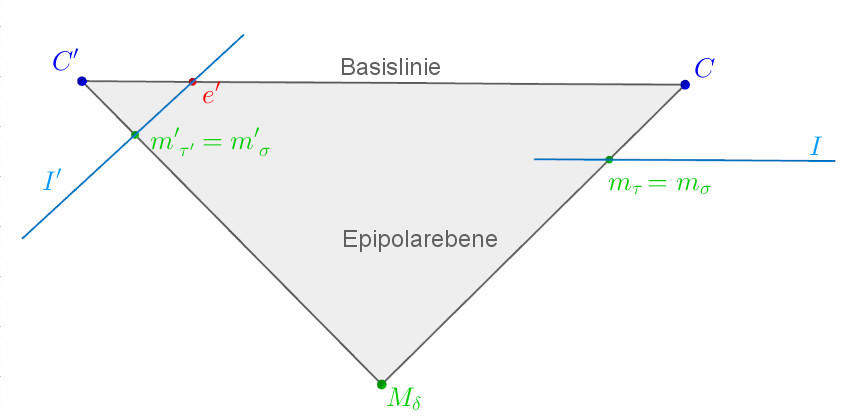
\includegraphics[width=\linewidth]{images/SynthetischesBeispielAufbauTopDown_beschriftet.png}
	\caption[Synthetisches Beispiel Top-Down-Ansicht]{In der Abbildung ist der vereinfachte Stereoaufbau in einer Top-Down-Ansicht zu sehen}
	\label{fig:aufbauMinimalTopDown}
	\endminipage\hfill
	\minipage{0.42\textwidth}
	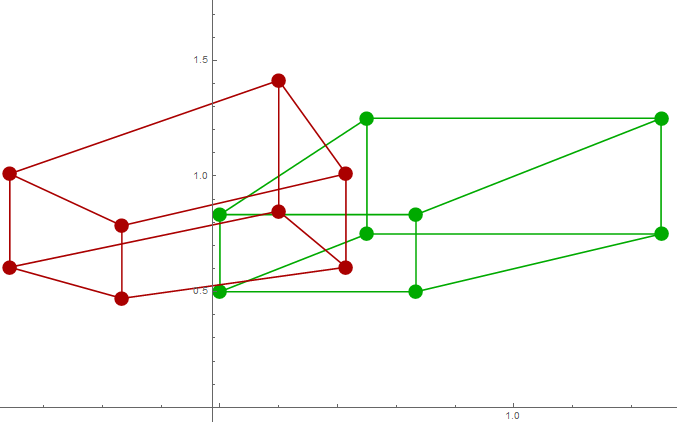
\includegraphics[width=\linewidth]{images/QuadrateMinimalBeispiel.png}
	\caption[Simulierte Abbildung eines Quaders auf zwei Kameras]{Simulierite Abbildung des Quaders auf die Kamera $C$ in Grün und auf $C'$ in Rot}
	\label{fig:AbbildungenMinimal}
	\endminipage\hfill
\end{figure}

\begin{figure}[!htb]
	\centering
	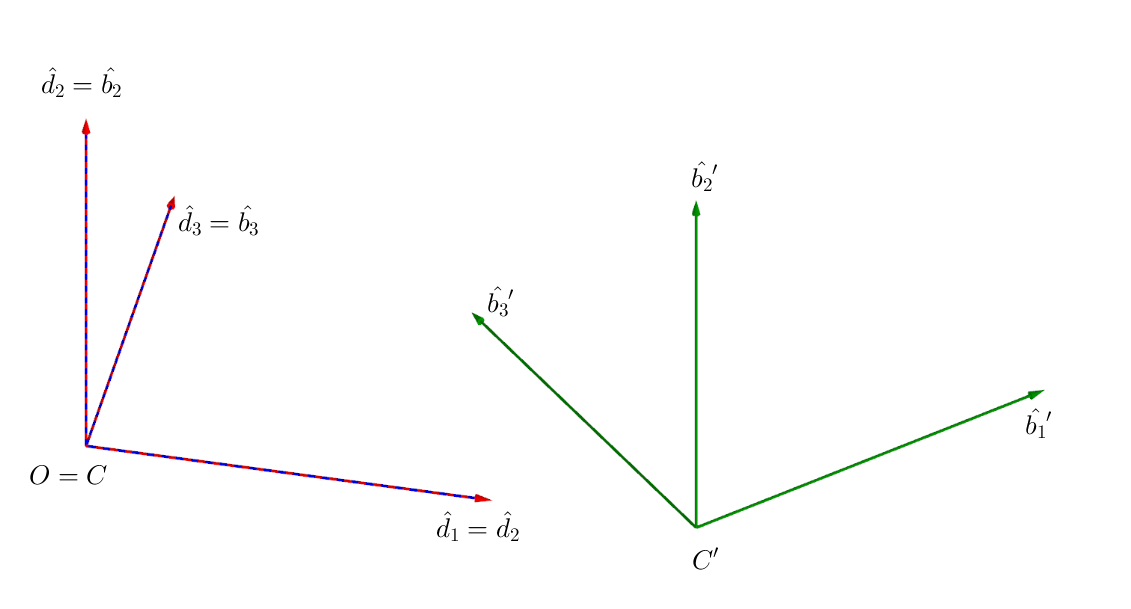
\includegraphics[width=.6\linewidth]{images/KS_Minimalbeispiel_beschriftet.png}
	\caption[Koordinatensysteme von $C$ und $C'$]{Abbildung der verschiedenen Kamerakoordinatensysteme, das Weltkoordinatensystem  $O$ ist zum Kamerakoordinatensystem $C$ deckungsgleich und $C'$  verschoben und rotiert.}
	\label{fig:KoordsystemeMinimal}
\end{figure}

%\begin{minipage}{\linewidth}
%	\centering
%	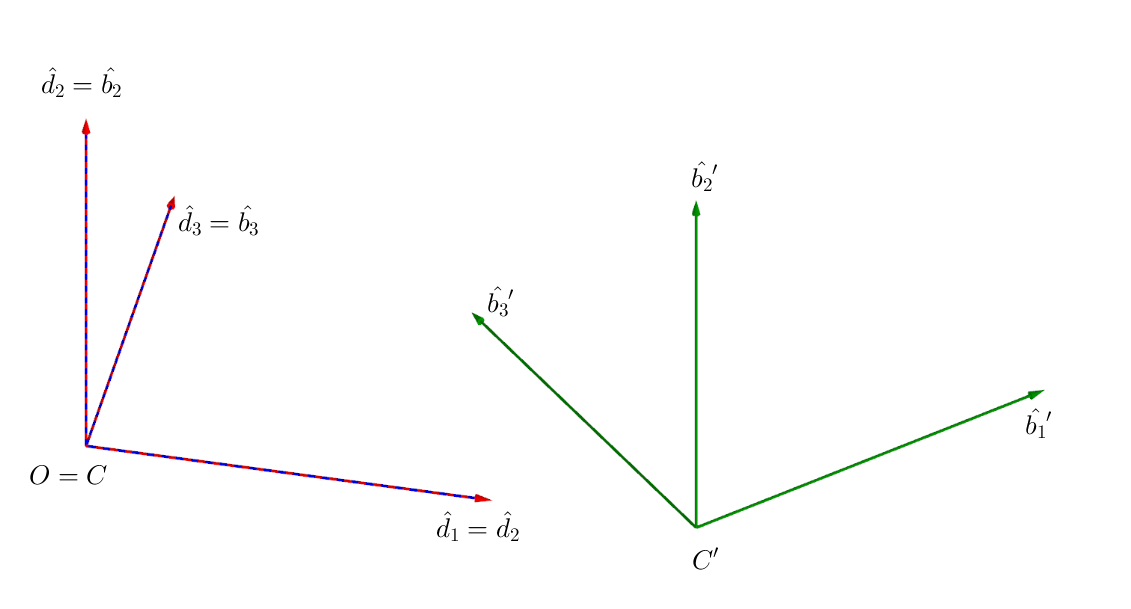
\includegraphics[width=.6\linewidth]{images/KS_Minimalbeispiel_beschriftet.png}
%	\captionof{figure}{Abbildung der verschiedenen Kamerakoordinatensysteme, das Weltkoordinatensystem  $O$ ist zum Kamerakoordinatensystem $C$ deckungsgleich und $C'$  verschoben und rotiert.}
%	\label{fig:KoordsystemeMinimal}
%\end{minipage}\\ \\

%
%Für die Stereokamerakalibrierung wird $C'$ relativ zur zu $C$ um einen Vektor \ensuremath{\vec{V'}} verschoben und anschließend um einen Winkel \ensuremath{\alpha} um die $b'_3$ Achse gedreht. Für die Rotation um \ensuremath{b'_3} wird eine Drehmatrix $D'$ aufgestellt.
Um die Eckpunkte des Quaders auf die Bildebenen von $C$ und $C'$ abbilden zu können, werden zunächst die Projektionsmatrizen $P$ und $P'$ aufgestellt. $C$ ist deckungsgleich mit dem Weltkoordinatensystem $(O,\delta)$. Es gilt also

\begin{gather}
R=\begin{pmatrix}
1&0&0\\
0&1&0\\
0&0&1
\end{pmatrix}\\
C=\begin{pmatrix}
0\\0\\0
\end{pmatrix}\\
T = R[I|-C]\\
T = \begin{bmatrix}
1&&0&&0&&C_1\\
0&&1&&0&&C_2\\
0&&0&&1&&C_3
\end{bmatrix}
\end{gather}. 

$C'$ dagegen ist gegenüber $C$ verschoben und rotiert. Als Beispiel wird eine Rotation um die $\hat{b_2}'$ Achse für $C'$ bestimmt. Somit gilt für $P'$:
%entlang $\hat{d_1}$ verschoben und um $\hat{b_2}$ rotiert. Somit ergibt sich für $T=[R|V]$ von $C$:

%Dabei gehen wir davon aus, dass $C$ weder rotiert noch verschoben ist, während $C'$ verschoben und rotiert ist.(Hier eher wieder allgemein bleiben C gegenüber O keine verönderung C' schon)





%Die entstandene Matrix \ensuremath{R'} beschreibt die Transformation $C'$ und somit auch die Transformation von Punkten des Koordinatensystems $(C,\beta)$ in $(C',\beta')$. Da $(C,\beta) = (O,\delta)$ ist, beinhaltet die Transformationsmatrix $R$ für $C$ weder eine Translation noch eine Rotation.

%Und für $R'=[D'|V']$ von $C'$ gilt:

\begin{gather}			
	R'= 
	\begin{pmatrix}
		\cos(\alpha)&0&\sin(\alpha)\\
		0&1&0\\
		-\sin(\alpha)&0&\cos(\alpha)
	\end{pmatrix}\\
	\vec{C'}= 
	\begin{pmatrix}
		1&0&0&-C'_1\\
		0&1&0&-C'_2\\
		0&0&1&-C'_3			
	\end{pmatrix}\\
	T'=R'[I|-C]\\
	T'=		\begin{pmatrix}
		\cos(\alpha)&0&-\sin(\alpha)\\
		0&1&0\\
		\sin(\alpha)&0&\cos(\alpha)
	\end{pmatrix} 
	\cdot
	\begin{pmatrix}
		1&0&0&-C'_1\\
		0&1&0&-C'_2\\
		0&0&1&-C'_3			
	\end{pmatrix}\\
	T'=
	\begin{pmatrix}
		\cos(\alpha)&0&-\sin(\alpha)&-C'_1\cos(\alpha)+C'_3\sin(\alpha)\\
		0&1&0&-C'_2\\
		\sin(\alpha)&0&\cos(\alpha)&-C'_1\sin(\alpha)-C'_3\cos(\alpha)\\
	\end{pmatrix}
\end{gather}\\

%\section{Berechnung der Projetkionsmatritzen }

%Neben den Eckpunkten des Quaders wird noch ein neunter Punkt $E_\delta$ außerhalb des Quaders platziert und zwar so, dass es zu keinen linearen Abhängigkeiten zwischen $E_\delta$ und den anderen Punkten kommt. 


Der Quader hat insgesamt acht Punkte, welche auf die Bildebenen der Kameras projiziert werden. Neben den Punkte des Quaders wird noch ein weiterer Punkt außerhalb des Quaders platziert und ebenfalls auf die Bildebenen projiziert. Mit insgesamt neun Punkten bei der Bestimmung der Fundamentalmatrix, wird die Wahrscheinlichkeit ein unterbestimmtes System aus der Koeffizientenmatrix $A$ zu bekommen minimiert. Ist $A$ unterbestimmt so besitzt sie Rang 7 und $F$ kann nicht eindeutig durch einen Sieben-Punkte-Algorithmus bestimmt werden\cite{HZ,LongQuan}. In dem hier berechneten Beispiel werden deswegen neun Punkte benutzt um sicherzugehen, dass $A$ Rang 8 besitzt und somit eindeutig bestimmt werden kann. Zur Bestimmung von $F$, wird der in Kapitel \ref{sec:HFE} aufgeführte Acht-Punkte Algorithmus angewandt.\\



%Mit insgesamt neun Punkten bei der Bestimmung der Fundamentalmatrix wird das Risiko einen Rangverlust durch lineare Abhängigkeiten minimiert\cite{HZ}. In Kapitel \ref{fig:Homographie} wurde geschildert, dass wenn die Koeffizientenmatrix $A$ einen Rang $\geq 8$ aufweist, $F$ mit Hilfe der Singulärwertzerlegung bestimmt werden kann\cite{HZ,Schwarz}. Besitz $A$ einen Rang von 7, so entspricht $A$ einer 7 $\times$ 9-Matrix. $A$ verhält sich wie eine Matrix, welche aus 7 statt 8 oder mehr Punktekorrespondenzen aufgestellt wurde. Das Verfahren die Fundamentalmatrix aus $A$ mit Rang 7 zu bestimmen, wird als der Sieben-Punkt-Algorithmus bezeichnet\cite{HZ,LongQuan}. In diesem Fall ist es immer noch möglich $F$ zu bestimmen, jedoch liefert die Bestimmung des Kerns von $F$ mit $A\cdot f = 0$ eine zweidimensionale Lösung in Form von $\alpha F_1 + (1- \alpha)F_2$\cite{HZ,LongQuan}. Nutzt man die aus der Singularität von $F$ folgende Bedingung, dass $det(F) = 0$ und somit  $\alpha F_1 + (1- \alpha)F_2 =0$, kann durch finden einer Lösung für $\alpha$ eine bis drei gültige Lösungen für $F$ gefunden werden\cite{HZ,LongQuan}. Im synthetischen Beispiel, soll dem Rangverlust von $A$ mit integrieren eines neunten Punktes entgegengewirkt werden, so das der acht-Punkte-Algorithmus für die spätere Bestimmung der Fundamentalmatrix angewendet werden kann.\\

% Sollte die Koeffizientenmatrix $A$ nur noch einen Rang von 7 statt 8 besitzen, so würden für $F$ zwei linear abhängige Lösungen entstehen.  Ist das der Fall, könnte trotzdem eine Lösung für $F$ ermittelt werden und zwar nach der Methode des sieben-Punkte-Algorithmus\cite{HZ}. Jedoch soll das im synthetischen Beispiel vermieden werden. \\

% auf die So kann vermieden werden, dass die später aufgestellt Koeffizientenmatrix, zum berechnen der Fundamentalmatrix, einen Rang kleiner als acht bekommt und somit zwei linear unabhängige Lösungen ausgibt\cite{HZ}. Ist das der Fall, könnte trotzdem eine Lösung für $F$ ermittelt werden und zwar nach der Methode des sieben-Punkte-Algorithmus\cite{HZ}. \\
%
%Die Eckp

%Im Unterkapitel \nameref{sec:MinimalFun} wird nochmal genauer drauf eingegangen, was das für $F$ bedeutet. Fürs erste wird festgelegt, dass insgesamt neun Punkte sich in der Szene befinden.

Um die neun Punkte auf die Bildebenen $(I,\tau)$ und $(I',\tau')$ zu projizieren, müssen neben den Transformationsmatrizen $R$ und $R'$ noch die Kameramatrizen $K_0$ und $K'_0$ festgelegt werden.


\begin{gather}		
K_0 =
\begin{bmatrix}
\zeta_{C}&0&0\\
0&\zeta_{C}&0\\
0&0&1\\
%0&0&1&0
\end{bmatrix}\label{eq:eq4.9}\\
K_0' =
\begin{bmatrix}
\zeta_{C'}&0&0\\
0&\zeta_{C'}&0\\
0&0&1\\
%0&0&1&0
\end{bmatrix}\label{eq:eq4.10}
\end{gather}

Da zunächst von gleichen Kameraauflösungen ausgegangen wird, gilt $\zeta = \zeta'$. Sind $R,R',K_0$ und $K'_0$ bekannt, können die Projektionsmatrizen gebildet und anschließend die Punkte auf die Bildebene projiziert werden. Die entstandenen Bilder sind in Abbildung \ref{fig:AbbildungenMinimal} zu sehen.  



\begin{gather}
%R=
%\begin{bmatrix}
%1&&0&&0&&v_1\\
%0&&1&&0&&v_2\\
%0&&0&&1&&v_3
%\end{bmatrix}\\
P = K_0\cdot R \\
P =
\begin{bmatrix}
\zeta_{C}&0&0\\
0&\zeta_{C}&0\\
0&0&1\\
%0&0&1&0
\end{bmatrix}\\
P' = K'_0 \cdot R'\\
P' =
\begin{bmatrix}
\zeta_{C'} \cos(\alpha)&0&\zeta_{C'} \sin(\alpha)&-\zeta_{C'} (v'_1\cos(\alpha)+v'_3\sin(\alpha) )\\
0&1&0&\zeta_{C'}-v'_2\\
\zeta_{C'}\sin(\alpha)&0&\zeta_{C'}\cos(\alpha)&-\zeta_{C'}(v'_1\sin(\alpha)+v'_3\cos(\alpha))\\
%0&0&0&0&1
\end{bmatrix}
\end{gather}



%\section{Transformation der Objektpunkte von Weltkoordinaten in Kamerakoordinaten}
%
%Die 3D-Punkte $A_\delta,B_\delta,C_\delta,D_\delta,A'_\delta,B'_\delta,C'_\delta,D'_\delta, E_\delta$, werden mit den Projektionsmatrizen \ensuremath{P} und \ensuremath{P'} auf die Bildebenen $I$ und $I'$ projizierten. Da das Sensorkoordinatensystem $(S,\sigma)$ deckungsgleich mit dem Bildebenenkoordinatesystem gesetzt wurde gilt das ein Bildebenpunkt $m_\tau$ gleich einem Sensorpunkt $m_\sigma$ ist. Die Bildaufnahme ist somit 
%Durch die Projektionsmatrix können die Punkte des Quaders auf die Bildebenen projiziert werden. Die entstandenen Bilder sind in Abbildung \ref{fig:AbbildungenMinimal} zu sehen. 

%Somit ist das Objekt auf den Bildebenen der virtuellen Kameras projiziert und der Szenenrekonstruktionsalgorithmus kann beginnen.



\section{Bildanalyse}
\label{sec:MinimalFun}

Der Szenenrekonstruktionsalgorithmus für das synthetische Beispiel ist in drei Abschnitte unterteilt. Zuerst wird aus den Punktekorrespondenzen die Fundamentalmatrix und die essentielle Matrix geschätzt. Mit Hilfe der essentiellen Matrix werden die extrinsischen Kameraparameter bestimmt, um so im letzten Schritt die Szenenpunkte durch Rückprojektion der Bildpunkte mit Hilfe der Kameraparameter rekonstruiert. 

%\subsection{Bestimmung der Abbildungsvorschriften}
\subsection{Bestimmung der extrinsischen Kameraparameter}

Zur Bestimmung der extrinsischen Kameraparameter werden in dem hier berechneten Beispiel neun korrespondierende Punkte bestimmt. Mittels des \textit{Epipolar-Constraint} aus Gleichung \ref{eq:Ep6} wird der Acht-Punkt-Algorithmus wie in Kapitel \ref{sec:8pointAlg} beschrieben angewandt, um die Fundamentalmatrix zu bestimmen.

\begin{gather}
	0=\vec{m'_\tau}^TK'^{-T}R' \left[ \vec{C'_\delta}-\vec{C_\delta}\right]_\times R^TK^{-1}\vec{m_\tau}\\
	=\vec{m'_\tau}F\vec{m_\tau}
	%0=\vec{m'_\tau}F\vec{m_\tau}
\end{gather}


Wie in Kapitel \ref{sec:EpiolarContraints} hergeleitet, bildet sich die essentielle Matrix aus:
\begin{gather}
	\vec{m'_\tau}^TK'^{-T}R' \left[ \vec{C'_\delta}-\vec{C_\delta}\right]_\times R^TK^{-1}\vec{m_\tau}=0\\
	\leadsto E = R' \left[ \vec{C'_\delta}-\vec{C_\delta}\right]_\times R^T		
\end{gather}

Um also $E$ aus $F$ zu bestimmen, gilt:
%Aus der Fundamentalmatrix und den bekannten intrinsischen Kameraparametern, wird die essentielle Matrix berechnet $E$, vergleiche Hierzu Gleichung \ref{eq:Ep8}


\begin{gather}
	 E= K'^T F K\\
    E= K'^T (K'^{-T}R' \left[ \vec{C'_\delta}-\vec{C_\delta}\right]_\times R^TK^{-1}) K\\
	E = R' \left[ \vec{C'_\delta}-\vec{C_\delta}\right]_\times R^T	
\end{gather}

%Tessentielle Matrix aus den normierten Bildebenenkoordinaten zu bestimmen.
%
%\begin{gather}
%	\vec{m'_\tau}^TK'^{-T}EK^{-1}\vec{m_\tau} = 0\\
%	\hat{m}'^T_{\tau'}.E.\hat{m}_\tau = 0 
%\end{gather}


%Wie in Kapitel \ref{sec:EpiolarContraints} hergeleitet, bildet sich die essentielle Matrix aus:
%\begin{gather}
%		\vec{m'_\tau}^TK'^{-T}R' \left[ \vec{C'_\delta}-\vec{C_\delta}\right]_\times R^TK^{-1}\vec{m_\tau}=0\\
%		\leadsto E = R' \left[ \vec{C'_\delta}-\vec{C_\delta}\right]_\times R^T		
%\end{gather}
Es wird davon ausgegangen, dass für $T = [R|-RC]$ von $C$ gilt, dass $T = [I|-0]$ ist. Die aus $E$ zu ermittelnde Matrix $T'$ beschreibt dann die Transformation von $C'$ relativ zu $C$\cite{HZ,Ferid}. Somit kann $E$ umformuliert werden zu:

\begin{gather}
	E = R'[\vec{C'_\delta} - \vec{C_\delta}]_\times R^T\\
	E = R'[\vec{C'_\delta} - 0]_\times I^T\\
	E = R'[\vec{C'_\delta}]_\times
\end{gather}


Um $R'$ und $[\vec{C'}_\delta]_\times$ zu bestimmen wird zunächst die essentielle Matrix \ensuremath{E}, mit Hilfe der Singulärwertszerlegung, in drei Matrizen zerlegt. 

\begin{gather}
E = U\Sigma V^T
\end{gather}

%Die Singulärwerte befinden sich in der mittleren Matrix $S = \text{diag}(\sigma_1,\sigma_2,\sigma_3)$ wieder.

Die Singulärwerte $\text{diag}(\sigma_1,\sigma_2,\sigma_3)$ der Matrix $\Sigma$ müssen die Bedingung erfüllen, dass $\Sigma = \text{diag}(1,1,0)$\cite{HZ,Ferid}. Wenn diese Bedingung nicht erfüllt ist, so wird sie erzwungen. Dazu wird Matrix $\Sigma$ aus der Sigulärwertszerlegung aus $E$ modifiziert\cite{HZ,Ferid}. 

\begin{gather}
	E' = U\text{diag}(1,1,0)V^T
\end{gather}  



%Damit die Matrix $E$ sich essentielle Matrix nennen darf, muss für zwei der Diagonaleinträge für die Singulärwerte gelten das $\sigma_1 = \sigma_2$ und $\sigma_3=0$ \cite{HZ,Ferid}. Da $T=[I|-C]$ und $T'=[R'|-R'C']$ gilt, setzt sich $E$ dementsprechend aus der Rotationsmatrize $R'$ und einer schiefsymmetrischen Matrix $S$ mit $S = [-R'C']_\times = [v]_\times$ zusammen\cite{HZ,phdextrinsicPara,Ferid}. 
%
%\begin{gather}
%E=[v]_\times R'\\
%S =[v]_\times\\
%E=SR'
%\end{gather}

$[C'_\delta]_\times$ ist schiefsymmetrisch und kann in $UZU^T$ zerlegt werden, wobei $U$ eine orthogonale Matrix ist und $Z$ eine block-diagonale Matrix\cite{HZ}. $R'$ wird in $UWV^T$ und $UW^TV^T$ zerlegt, wobei $W$ eine schiefsymmetrische Matrix ist\cite{Ferid,HZ,phdextrinsicPara}.%Zur Schätzung von $S$ und $R$ werden die schiefsymmetrische Matrix \ensuremath{W} und die Blockdiagonale Matrix \ensuremath{Z} eingeführt



\begin{gather}
W = \begin{pmatrix}
0&-1&0\\
1&0&0\\
0&0&1
\end{pmatrix} \;\;\;
Z=
\begin{pmatrix}
0&1&0\\
-1&0&0\\
0&0&0
\end{pmatrix}
\end{gather}

%Mit dem Ergebnis der SVD von $E$ mit \ensuremath{\text{SVD}(E) = USV^T} lassen 

Somit lassen sich die folgenden Lösungmöglichkeiten für $[C'_\delta]_\times$ und $R_1$ und $R_2$ aufstellen\cite{HZ,Ferid}.


\begin{gather}
[C'_\delta]_\times = \pm \,UZU^T \\
R_1' = UW^TV^T \;\;\;\; R_2' = UWV^T
\end{gather}\\


%Um sicher zu gehen, dass es sich bei \ensuremath{R_1}' und \ensuremath{R_2}' auch um gültige Rotationsmatrizen handelt, kann eine Probe durchgeführt werden.  \ensuremath{R\cdot R^T=I_{3\times3}} sein. \ensuremath{I_{3\times3}} steht für die 3$\times$3-Einheitsmatrix.

$[C'_\delta]_\times$ ist eine schiefsymmetrische Matrix, welche die Information für den noch gesuchten Translationsanteil $v = -R'C'$ beinhaltet. Ohne zusätzliche Informationen kann $v$ nur bis zu einer Skaleninvarianz genau bestimmt werden\cite{HZ,Ferid,phdextrinsicPara}. Durch die Modifizierung der Singulärwerte von $E$ gilt für $\parallel v \parallel = 1$\cite{HZ,Ferid}. Das bedeutet, dass es sich bei dem Translationsvektor $v$ lediglich um den normierten Richtungsvektor zwischen $C$ und $C'$ handelt\cite{KIT}. Um $v$ aus $[C'_\delta]_\times$ zu extrahieren, wird der Kern von $[C'_\delta]_\times$ bestimmt

%Aufgrund der Tatsache, dass die essentielle Matrix eine Größe des projektiven Raumes darstellt und deshalb nur bis auf einen Skalierungsfaktor definiert ist, kann lediglich die Richtung, nicht aber die Läange des Translationsvektors bestimmt werden\cite{KIT}

\begin{gather}
[C'_\delta]_\times \cdot v = v \times v = 0
\end{gather} 
.

Die Skaleninvarianz bewirkt, dass es bei der Rekonstruktion die Größe der Objekte von ihrer Originalgröße abweichen, da es sich bei $v$ nur um den normierten Richtungsvektor der Ursprünglichen Strecke handelt. Die Abbildung \ref{fig:scale3} zeigt die Auswirkungen der Skaleninvarianz auf die später rekonstruierte Szene. \\

Letztendlich können für die Rekonstruktion der extrinsischen Kameraparameter vier mögliche Lösungen für $T$ in Form von $T = R[I|-C]$, wie in Gleichung \ref{eq:trafo} in Kapitel \ref{sec:CameraModels} definiert, gefunden werden\cite{HZ,Ferid,phdextrinsicPara}. $\lambda v$ heißt dabei, dass sowohl $v$ also auch alle Vielfache von $v$ Lösungen sein können, was durch die Skaleninvarianz der Resultate bedingt ist\cite{HZ,Ferid,phdextrinsicPara}. 

\begin{gather}
T' = [UWV^T|+\lambda v] \;\;\; \text{oder} \;\;\;[UW^TV^T|+\lambda v]\\
\textit{oder}\;\;\; [UWV^T|-\lambda v] \;\;\; \text{oder} \;\;\;[UW^TV^T|-\lambda v]
\end{gather}

Die Abbildungen \ref{fig:T_1} und \ref{fig:T_2} stellen schematisch die vier verschiedenen Transformationsmöglichkeiten von $T'$ dar. Die richtige Lösung $T$ ist diejenige, bei der das Abbild der Objekte vor den Kameras liegt.\\\\


\begin{figure}[!htb]
	\minipage{0.5\textwidth}
	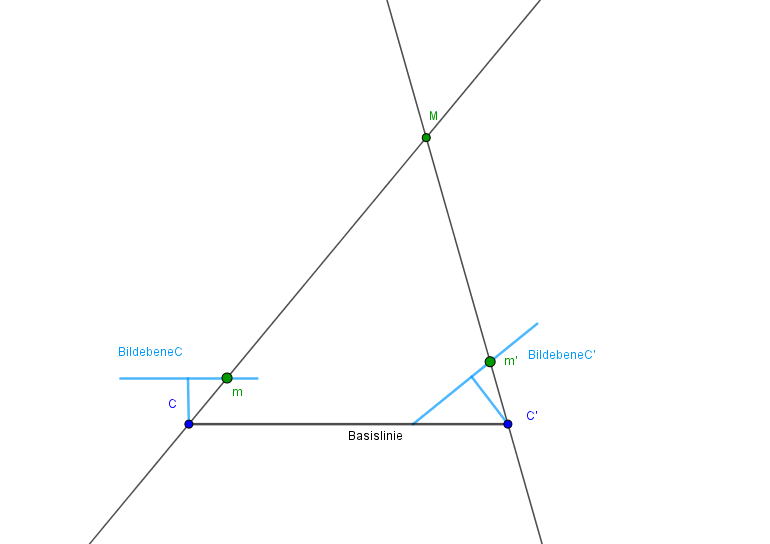
\includegraphics[width=\linewidth]{images/P_Solution_one.png}
%	\caption[Bestimmung extrinsischer Kameraparameter erste Lösung]{a)}
%	\label{fig:T_1}
	\endminipage\hfill
	\minipage{0.52\textwidth}
	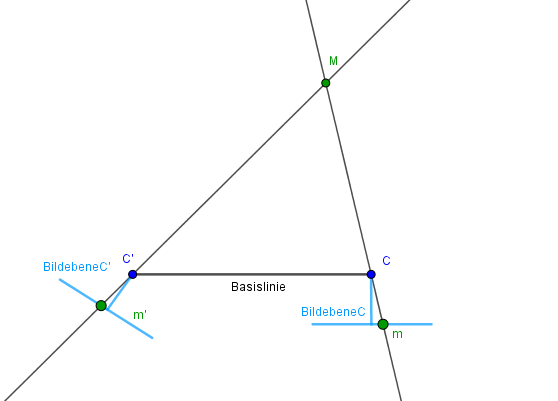
\includegraphics[width=\linewidth]{images/P_Solution_two.png}
	%\caption[Bestimmung extrinsischer Kameraparameter zweite Lösung]{b)}
%	\label{fig:T_2}	
	\endminipage\hfill	
	\caption[Bestimmung extrinsischer Kameraparameter Lösung eins und zwei]{In den ersten beiden Abbildungen kommt es zu einer Umkehrung der Basisline.}
	\label{fig:T_1}
\end{figure}
\begin{figure}[!htb]
	\minipage{0.52\textwidth}
	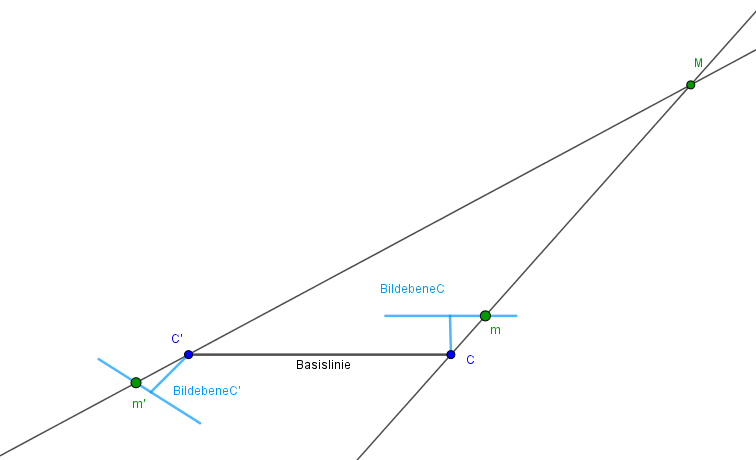
\includegraphics[width=\linewidth]{images/P_Solution_three.png}
%	\caption[Bestimmung extrinsischer Kameraparameter dritte Lösung]{c)}
%	\label{fig:T_3}
	\endminipage\hfill
	\minipage{0.5\textwidth}
	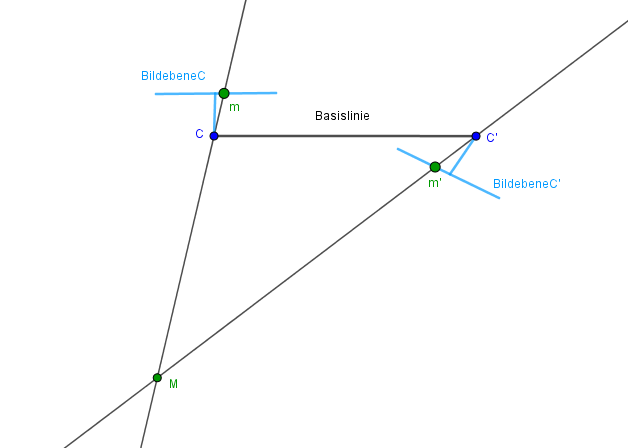
\includegraphics[width=\linewidth]{images/P_Solution_four.png}
	%\caption[Bestimmung extrinsischer Kameraparameter vierte Lösung]{d)}
%	\label{fig:T_4}
	\endminipage\hfill
	\caption[Bestimmung extrinsischer Kameraparameter Lösung eins und zwei]{In den beiden Abbildungen wird $C'$ und $180^\circ$ gedreht}
	\label{fig:T_2}
%	\caption[Alle vier Lösungen im Überblick]{Die Abbildungen a, b, c und d veranschaulichen, welche Bilder aus den vier Lösungen entstehen. In den Abbildungen a und b kommt es zu einer Umkehrung der Basisline. In den Abbildungen c und d wird $C'$ und $180^\circ$ gedreht}
\end{figure}
\pagebreak

%Zur Bestimmung der Abbildungsvorschrift wird die Fundamentalmatrix $F$ aus den korrespondierenden Punkten bestimmt. Die korrespondierenden Punkte sind Bildpunkte auf den verschiedenen Bildebenen eines gleichen Ursprungspunktes. Anhand des in Kapitel \ref{sec:HFE} beschriebenen 8-Punkte-Algorithmus, wird $F$ bestimmt. Über $F$ wird die essentielle Matrix $E$, mit den aus Kapitel \ref{sec:HFE} ermittelt Bedingung aus Gleichung \ref{eq:Ep7}, bestimmt.\\
%
%In dieser Arbeit wird angenommen, dass die Kameras zuvor einzeln Kalibriert wurden und die intrinsischen Kameraparameter bereits bekannt sind. Für die Bestimmung der extrinsischen Kameraparameter wird ein Ansatz verfolgt, in welchen die essentielle Matrix zum Einsatz kommt. Die essentielle Matrix ist eine Spezialform der Fundamentalmatrix und beschreibt den \textit{Epipolar-Constraint}, vlg \ref{eq:Ep7}, zwischen den normierten Bildebenenkoordinaten\cite{HZ,Elements,ZZGXr,Zhang2014,Ferid}. 
%
%\begin{gather}
%\hat{m}'^T_{\tau'}.E.\hat{m}_\tau = 0 
%\end{gather}
%
%Sind $F$ und Kameramatrizen $K$ und $K'$ bekannt, kann die essentielle Matrix wie in Kapitel \ref{eq:Ep7} gezeigt aus $F$ bestimmt werden. Die essentielle Matrix ist eine Fundamentalmatrix, welche zu einem paar normierter Projektionsmatrizen $\hat{P}$ mit $\hat{P} = [I|0]$ und $\hat{P}'$ mit $\hat{P}'= [R'|V']$ korrespondierend ist\cite{HZ,Zhang2014,ZZGXr,Ferid}. Um die Projektionsmatrix $P'=K'[R'|V']$ auf die normierte Form zu bringen, müssen die intrinsischen Parameter für $K'$ bekannt sein\cite{HZ}. 
%
%\begin{gather}
%	m'_{\tau} = P' \cdot M_\delta\\
%	m'_{\tau} = K'[R'|C'] \cdot M_\delta\;\; | \cdot K'^{-1}\\
%	\end{gather}
%	
%Die Inverse $K^{-1}$ wird auf beiden Seiten der Gleichung von links multipliziert\cite{HZ}.
%
%\begin{gather}
%	K'^{-1} \cdot m'_{\tau} = K'^{-1} \cdot K'[R'|C'] \cdot M_\delta\\
%	\hat{m}'_{\tau} = [R'|C'] M_\delta
%\end{gather}
%
%$M_\delta$ ist ein Objektpunkt im 3D-Raum, welcher mit $P'$ zum Bildebenenpunkt $m'_{\tau'}$ abgebildet wird. Nach der Normierung, wird $\hat{m}'_{\tau}$ als normierte Bildebenenkoordinate bezeichnet und die entstandene Projektionsmatrix $P' = [R'|C']$ als normierte Projektionsmatrix\cite{HZ,Ferid}. $E$ wird aus $F$ bestimmt mit:

%\begin{gather}
%E = K'^TFK
%\end{gather}

%det(E) = det(t×) det(R) = 0. Somit enth¨alt die Essentialmatrix
%nur zwei linear unabh¨angige Zeilen- oder Spaltenvektoren und hat den
%Rang4 Rg(E) = 2.
%Wie die Fundamentalmatrix muss auch die essentielle Matrix einen Rang von 2 haben. Des Weiteren darf eine 3 $\times$ 3-Matrix nur dann als essentielle Matrix bezeichnet werden, wenn die Singulärwerte, bestimmte Merkmale aufweisen. So müssen zwei der drei Singulärwerte gleich und die dritte null sein\cite{HZ}. Des Weiteren muss für die Determintante gelten, dass $det(E) = 0$ ist und die Quadratwurzel der Eigenwerte müssen wieder die Singulärwerte ergeben\cite{Ferid}. 

%\subsection{Bestimmung der extrinsischen Kameraparameter}

%(Noch einen Ansatz einbauen wie man die richtige Lösung algorithmisch auswertet? Im implementierte Algorithmus der arbeit wurden die Vier Lösungen jeweils rekonstruiert und alle ergebnisse ausgegeben.)

\subsection{Szenenrekonstruktion durch Triangulation}

Als Triangulierung wird in der Computer Vision die Bestimmung eines 3D-Objektpunktes aus korrespondierenden Bildpunkten bezeichnet. Als Voraussetzung für die Rekonstruktion müssen die jeweiligen korrespondierenden Bildpunkte und die Kameraparameter der einzelnen Kameras bekannt sein. Die Triangulierung funktioniert wie eine umgekehrte Projektion der Bildpunkte auf der Bildebene in einen Objektpunktes im Raum. Zwei Geraden, welche jeweils durch die Projektionszentren und den zu rekonstruierenden Bildpunkten gehen,  treffen sich im Raum. Der Schnittpunkt beider Geraden bildet den zu den Bildpunkten gehörenden Ursprungspunkt, wie in Abbildung \ref{fig:TriangulationOptimal} schematisch dargestellt ist.  \\\\


%wird das Rekonstruieren der Ursprünglichen 3D-Objektpunkte durch eine Rückprojektion vom jeweiligen Projektionszentrum der Kameras durch ihre Bildpunkte bezeichnet. Im synthetischen Beispiel wird durch einfache Schnittpunktberechnung derjenigen Geraden, welche durch die jeweiligen Projektionszentren und deren Bildpunkte auf deren Bildebenen gehen, der Ursprungspunkt im Raum rekonstruiert.\\


%\begin{minipage}{\linewidth}
%	\centering
%	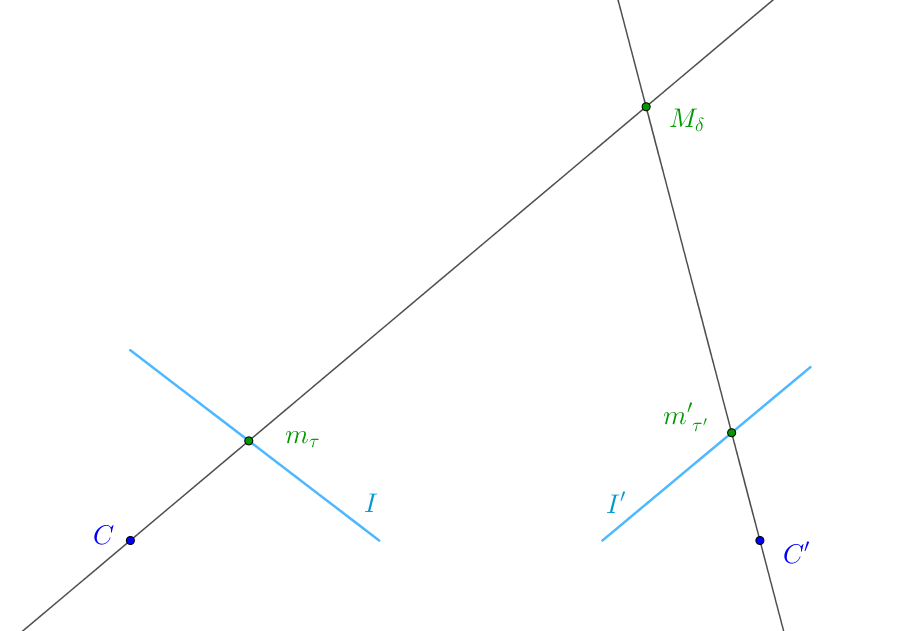
\includegraphics[width=0.8\linewidth]{images/optimaleTriangulierung.png}
%	\captionof{figure}{Optimale Triangulierung: Beide Geraden Treffen sich in einem Punkt im 3D-Raum} 
%	\label{fig:TriangulationOptimal}
%\end{minipage}\\ \\

\begin{figure}[!htb]
	\centering
	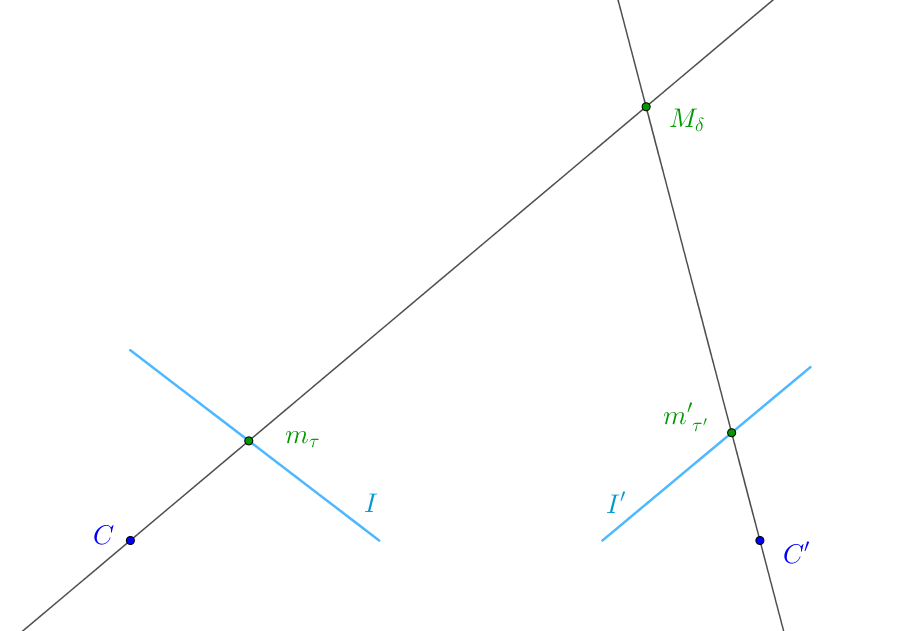
\includegraphics[width=0.8\linewidth]{images/optimaleTriangulierung.png}
	\caption[Einfache Triangulation]{Optimale Triangulierung: Beide Geraden Treffen sich in einem Punkt im 3D-Raum} 
	\label{fig:TriangulationOptimal}
\end{figure}

%bei der Szenenrekonstruktion realen Stereoaufnahmen kann eine Triangulation nicht so ohne weiteres durchgeführt werden. Bei einer Bildaufnahme mit Kameras, kommt es nicht selten vor, dass 
%
%In Realbildern, können Bildfehler wie beispielsweise Rauschen nicht vermieden werden, des Weiteren können korrespondierende Punkte nicht immer exakt auf den Pixel genau bestimmt werden.
% 
%Anders hingegen wäre es in einem realen Beispiel mit korrespondierenden Punkten, welche Beispielsweise über einen \textit{SURF}- Algorithmus detektiert wurden\cite{Mandun}. Diese Fehler führen dazu, dass wenn ein Schnittpunkt der Geraden durch die vermeintlichen korresponiderenden Punkte nicht gefunden werden kann, da die Geraden sich sehr wahrscheinlich nicht in einem Punkt treffen werden\cite{Mandun,HZ}. 
%
%
%\begin{minipage}{\linewidth}
%	\centering
%	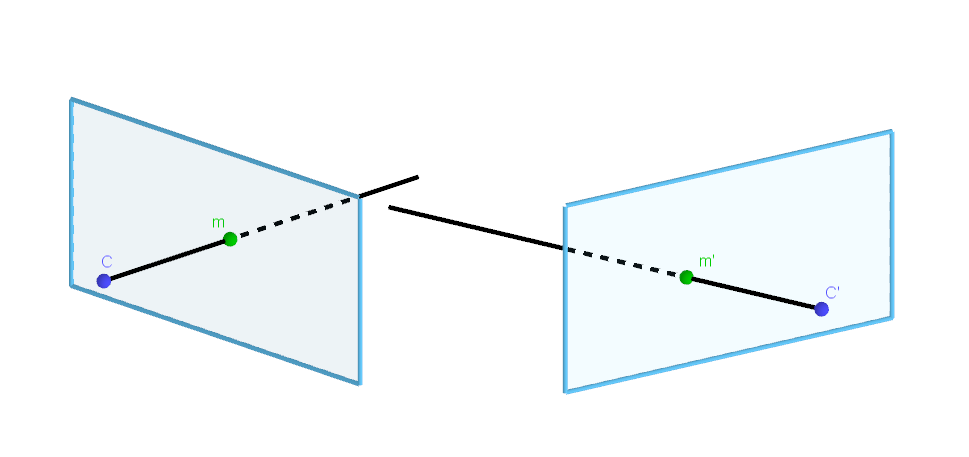
\includegraphics[width=0.8\linewidth]{images/problemTriangulation.png}
%	\captionof{figure}{Durch Ungenauigkeiten in der korrespondierenden Punkte, verfehlen sich die Linien und es kommt zu keinem Schnittpunkt} 
%\end{minipage}\\ 
%
%Für diese Fälle gibt es mehrere Näherungsverfahren, wovon eines, im Kapitel \nameref{sec:sampson}, im Realbeispiel eingeführt wird\cite{HZ}. In diesem Minimalbeispiel tritt der optimale Fall ein. Das bedeutet, dass ein zu Bildpunkt $m$ korrespondierender Bildpunkt $m'$ auf der zu $m$ korrespondierenden Epipolarlinie $l'$ liegt und somit garantiert ist, dass sich die Geraden $\overline{mM}$ und $\overline{m'M}$ auf jedenfall in einem gemeinsamen Punkt schneiden.
%
% Um den Schnittpunkt beider Geraden zu berechnen, werden zum einen die Bildpunkte  $A_\tau,B_\tau,C_\tau,D_\tau,A2_\tau,B2_\tau,C2_\tau,D2_\tau$ und $A_{\tau'},B_{\tau'},C_{\tau'},D_{\tau'},A2_{\tau'},B2_{\tau'},C2_{\tau'},D2_{\tau'}$, sowie die korrekt ermittelte Projektionsmatrix $P'$ von zuvor benötigt. 

Im synthetischen Beispiel wird mit reinen Daten gearbeitet. Das heißt, die Bildpunkte wurden mathematisch von ihrem Ursprungspunkt im Raum berechnet und sind somit frei von Verfälschungen durch äußere Einflüsse. Ein zum Bildpunkt $m_\tau$ korrespondierender Bildpunkt $m'_{\tau'}$ liegt genau auf der zu $m_\tau$ korrespondierenden Epipolarlinien $l'$. Somit ist garantiert, dass sich die Bildpunkte $m_\tau$ und $m'_{\tau'}$ bei einer Rückprojektion in einem Punkt $M_{0,\delta}$ im Raum treffen. Durch die zuvor erwähnte Skaleninvarianz der extrinsischen Kameraparameter handelt es sich bei $M_{0,\delta}$ jedoch noch nicht um den eigentlichen Ursprungspunkt $M_\delta$. \\

%Um die Rekonstruktion im synthetischen Beispiel so nah wie möglich an einem realen Beispiel zu halten, wird davon ausgegangen, dass nur die Kameraparameter und die jeweiligen Bildkoordinaten bekannt sind.\\


Vor der Bestimmung der extrinsischen Kameraparameter wurde festgesetzt, dass $T = [I|-0]$ die Translationsmatrix von $C$ ist. Somit gilt für die Projektionsmatrix von $C$, dass $P= K_0T =K_0[I|-0]$ ist. Die Projektionsmatrix $P'$ für $C'$ setzt sich aus einer der Lösungen von $T'$ und der Kameramatrix $K_0'$ zusammen, sodass gilt $P'=K_0'T' = K[R'|-RC]$.\\

Um eine Gerade von den Projektionszentren $C$ und $C'$ durch die jeweiligen Bildpunkte bilden zu können, müssen die Positionen von $C$ und $C'$ bekannt sein. Da die Koordinatensysteme $(C,\beta)$ und $(O,\delta)$ deckungsgleich sind, und $P = K_0[I|-0]$ ist, gilt $C = (0,0,0)^T$.  Um $C'$ aus $T' = R'[R'|-R'C']$ zu bestimmen wird der Translationsvektor $-R'C'$ aus $T'$ mit dem transponierten Rotationsmatrix $R'^T$ aus $T'$ multipliziert.

\begin{gather}
	C' =  R'^T \cdot -R'C' 
\end{gather}

%Nachdem die Position der Kamerazentren $C$ und $C'$ bekannt sind werden die Bildpunkte noch in Koordinaten bezüglich der jeweiligen Kamerakoordinatensysteme $(C,\beta)$ und $(C',\beta')$ transformiert. Dazu werden die zweidimensionalen Bildpunkte $m_\tau$ und $m_\tau'$ um den jeweiligen Abstand des Projektionszentrums zur Bildebene, sprich $\zeta$ und $\zeta'$, erweitert.
%

Die zweidimensionalen Bildpunkte werden mit den bekannten Brennweiten $\zeta$ und $\zeta'$ aus $K_0$ und $K_0'$ zu einer dreidimensionalen Koordinate erweitert.

\begin{gather}
	\begin{pmatrix}
	m_{\tau x}\\
	m_{\tau y}\\
	\end{pmatrix} \leadsto 
		\begin{pmatrix}
	m_{\tau x} \\
	m_{\tau y}\\
	\zeta
	\end{pmatrix}\\
		\begin{pmatrix}
	m'_{\tau' x}\\
	m'_{\tau' y}\\
	\end{pmatrix} \leadsto 
	\begin{pmatrix}
	m'_{\tau' x} \\
	m'_{\tau' y}\\
	\zeta
	\end{pmatrix}	
\end{gather}

Danach werden für die Rückprojektion zwei Geradengleichungen aufgestellt. Eine Gerade geht durch $C$ und $	\begin{pmatrix}
m_{\tau x} \\
m_{\tau y}\\
\zeta
\end{pmatrix} $ die zweite Gerade geht durch die Punkte $C'$ und $	\begin{pmatrix}
m'_{\tau' x} \\
m'_{\tau' y}\\
\zeta'
\end{pmatrix}$. Anschließend wird aus den zwei Geraden der Schnittpunkt $M_{\delta,0}$ im Raum bestimmt. $C$ und $C'$ sind aus Sicht des Weltkoordinatesystems $(O,\delta)$ definiert. $m'_{\tau'}$ wird in Koordinaten bezüglich des Kamerakoordinatesystem $(C,\beta)$ transformiert mit $m'_\beta = \begin{bmatrix}
R[I|-C']
\end{bmatrix}^{-1} \cdot m'_{\tau'}$.



\begin{gather}
	 g:= \vec{C} + t \cdot 
	\begin{pmatrix}
	 	\vec{C} -	
	\begin{pmatrix}	
	m_{\beta x} \\
	m_{\beta y}\\
	\zeta
	\end{pmatrix}
 \end{pmatrix} \\
g' := \vec{C'} + t \cdot 
\begin{pmatrix}
	\vec{C'} -
	\begin{pmatrix}
	m'_{\beta x} \\
	m'_{\beta y}\\
	\zeta'
	\end{pmatrix}
\end{pmatrix}
\end{gather}


 
%
%Nun muss für jedes Linienpaar eine Lösung für $t$ und $t'$ gefunden werden und die Lösungen in die Gleichungen 4.65 und 4.66 eingesetzt werden. Es sollte für beide Gleichungen die selbe Lösung für den rekonstruierten Punkt $A$ im Raum ergeben. Die Lösung entspricht meist noch nicht exakt dem eigentlichen Ergebnis, das liegt an der zuvor erwähnten Skaleninvariants der Rekonstruktion der exterenen Kameraparameter. 

Bei den zuvor ermittelten extrinsischen Kameraparametern ist der Translationsvektor skaleninvariant. Dies führt dazu, dass der rekonstruierte Objektpunkt $M_{\delta,0}$ nach der Szenenrekonstruktion noch nicht dem Ursprünglichen $M_\delta$ entsprechen muss. Dementsprechend wird als letzter Schritt die rekonstruierte Szenen anhand einer bekannten Referenzgröße skaliert. Als Referenzgröße kann beispielsweise ein zuvor abgemessener Abstand zwischen zwei Punkten in der Szene dienen. Im synthetischen Aufbau sind beispielsweise die Abstände zwischen den Originalbildpunkten bekannt. Die Abbildung \ref{fig:scale3} zeigt die Szene des Quaders mit unterschiedlichen Skalierungen. Die Abbildung \ref{fig:Quader1} zeigt die rekonstruierte Szene des synthetischen Beispiels auf uhre Ursprungsgröße skaliert.

%ihrer Originalgröße entsprechen. 
%
%Es wird noch ein Skalierungsfaktor benötigt, welcher die Szene auf Originalgröße skaliert. Hierfür ist es in einer Realszene ratsam, wenn man zuvor von zwei Punkten in Szene den Abstand zueinander abmisst, um anhand dessen einen Skalierungsfaktor zu berechnen. Im hier beschriebenen Minimalbeispiel sind die Originalkoordinaten der Objektpunkte im Raum bekannt, weshalb hier nach dem passenden Vielfachen der Rekonstruierten Punkte gesucht werden kann.
%
% Da die Verhätnisse der Abstände der Punkte zueinander bei der skalierung beibehalten wird, kommt zu keinen Verfälschungen des Objektes, da die Rotationen der beiden Kameras unangetastet bleibt. 


\begin{figure}[!htb]
	\minipage{0.40\textwidth}
	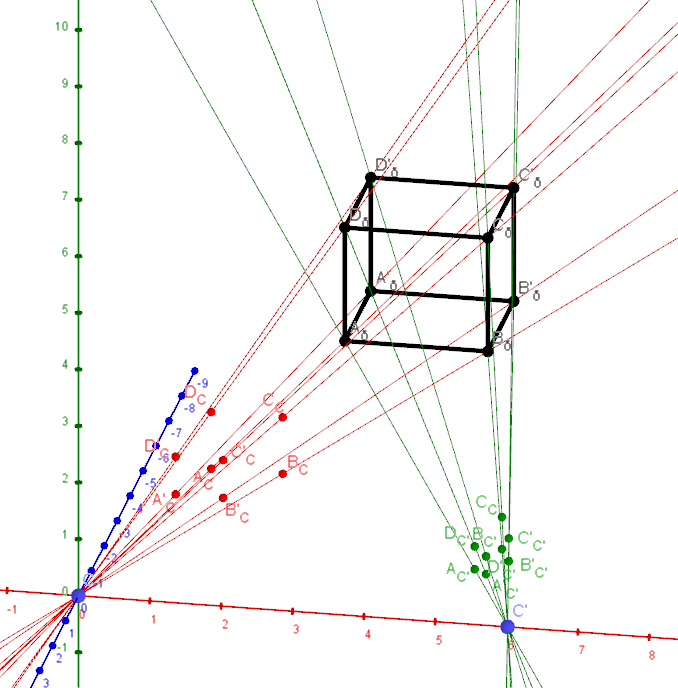
\includegraphics[width=\linewidth]{images/ScaleInvariance_1.png}
%	\caption{}
%	\label{fig:scale1}
	\endminipage\hfill
	\minipage{0.40\textwidth}
	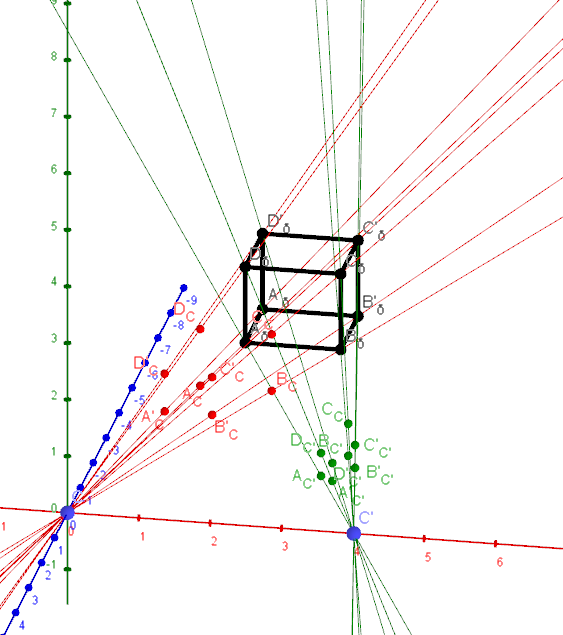
\includegraphics[width=\linewidth]{images/ScaleInvariance_2.png}
%	\caption{}
%	\label{fig:scale2}
	\endminipage\hfill
\end{figure}

\begin{figure}[!htb]
	\centering
	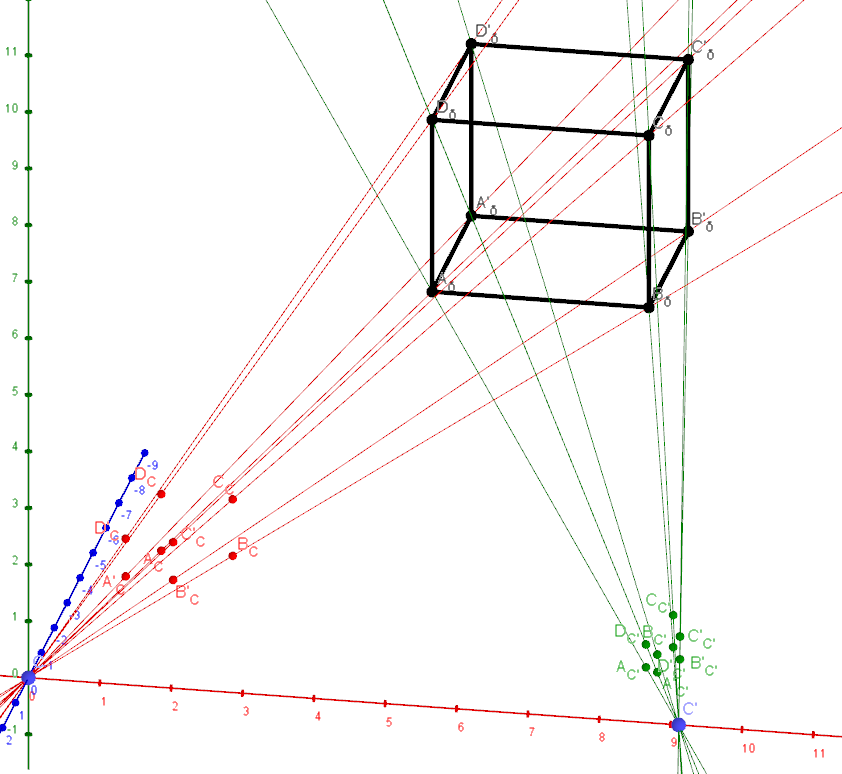
\includegraphics[width=0.40\linewidth]{images/ScaleInvariance_3.png}
	\caption[Skalierung der Rekonstruierten Szene]{Veranschaulichung der Skaleninvarianz und dessen Auswirkung auf die geometrische Form und Größe der Objekte} 
	\label{fig:scale3}
\end{figure}
\pagebreak



\begin{figure}[!htb]
	\minipage{0.42\textwidth}
	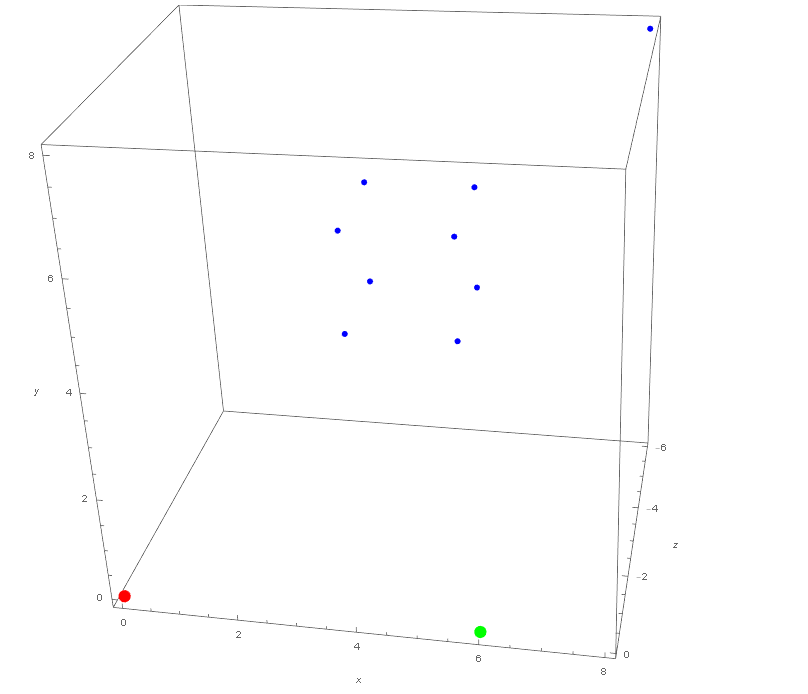
\includegraphics[width=\linewidth]{images/MinimalBeispiel_reconstructed.png}
	%\caption{}
	\endminipage\hfill
	\minipage{0.42\textwidth}
	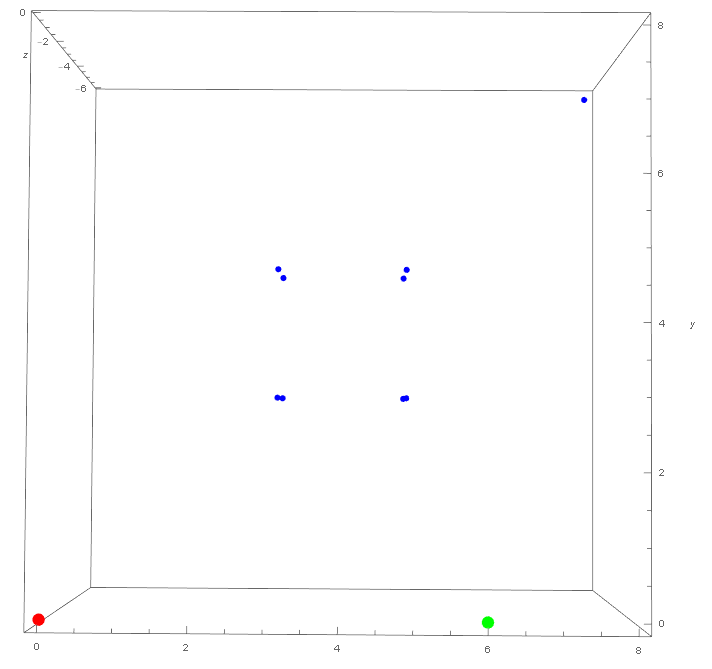
\includegraphics[width=\linewidth]{images/MinimalBeispiel_reconstructed_3.png}
%	\caption{}
	\endminipage\hfill
	\caption[Programmplot der rekonstruierten Szene]{Der rote Punkt stellt die Postion von $C$ dar, der grüne steht für die Position von $C'$ relativ zu $C$. Die blauen Punkte stellen den rekonstruierten Quader und den extern platzierten neunten Punkt da. Die Abbildungen entstand aus dem in \textit{Mathematica}\cite{Mathematica} implementierten Algorithmus.}
		\label{fig:Quader1}
\end{figure}
\pagebreak


